% This is samplepaper.tex, a sample chapter demonstrating the
% LLNCS macro package for Springer Computer Science proceedings;
% Version 2.20 of 2017/10/04
%
\documentclass[runningheads]{llncs}

\usepackage{graphicx}
\usepackage{ae,aecompl}
\usepackage[utf8]{inputenc}
\usepackage[english]{babel}
\usepackage{verbatim}
\usepackage{graphicx}
\usepackage{amsfonts}
\usepackage{amsmath}
\usepackage{amssymb}
\usepackage{stmaryrd}
\usepackage{amstext}
\usepackage{bm} 
\let\proof\relax
\let\endproof\relax
\usepackage{amsthm}
\usepackage{siunitx}
\usepackage{mathrsfs}
\usepackage{wrapfig}
%\usepackage{minted}
\usepackage{algorithm}
\usepackage{algpseudocode}
\usepackage{semantic}
\usepackage[dvipsnames]{xcolor}
\usepackage{paralist}
\usepackage{cite}
\usepackage{cleveref}
\usepackage{url}
\usepackage{todonotes}
\usepackage{cleveref}
% Used for displaying a sample figure. If possible, figure files should
% be included in EPS format.
%
% If you use the hyperref package, please uncomment the following line
% to display URLs in blue roman font according to Springer's eBook style:
% \renewcommand\UrlFont{\color{blue}\rmfamily}
% Comments

% Paper specific notation

\setlength{\intextsep}{10pt}

\newcommand{\load}{\ensuremath{\mathit{load}}}
\newcommand{\env}{\ensuremath{\mathit{env}}}
\newcommand{\psu}{\ensuremath{\mathit{psu}}}
\newcommand{\plant}{\ensuremath{\mathit{plant}}}
\newcommand{\ctrl}{\ensuremath{\mathit{ctrl}}}
\newcommand{\fref}{\ensuremath{\mathit{ref}}}
\newcommand{\xaft}{\ensuremath{\mathit{xaft}}}

\newcommand{\inputV}{v}
\newcommand{\consistent}{\ensuremath{\mathit{Consistent}}}
\newcommand{\remaining}{\ensuremath{\mathit{Remaining}}}
\newcommand{\dontcare}{\_}
\newcommand{\defined}{\ensuremath{\mathit{defined}}}
\newcommand{\undefined}{\ensuremath{\mathit{undefined}}}
\newcommand{\properties}{P}
\newcommand{\satisfies}{\vDash}
\newcommand{\simulator}{\mathcal{A}}
\newcommand{\Induced}[2]{\llbracket #1 \rrbracket_{#2}}
\newcommand{\timebase}{\setreal_{\geq 0}}
\newcommand{\stateset}[1]{S_{#1}}
\newcommand{\runstate}[1]{S^{R}_{#1}}
\newcommand{\state}[1]{s_{#1}}
\newcommand{\inputs}[1]{U_{#1}}
\newcommand{\inputvar}[1]{u_{#1}}
\newcommand{\outputs}[1]{Y_{#1}}
\newcommand{\outputvar}[1]{y_{#1}}
\newcommand{\values}{\mathcal{V}}
\newcommand{\true}{\mathit{true}}
\newcommand{\false}{\mathit{false}}
\newcommand{\feedthrough}[1]{D_{#1}}
\newcommand{\reactivity}[1]{R_{#1}}
%\newcommand{\finit}[1]{\mathtt{init}_{#1}}
\newcommand{\fset}[1]{\mathtt{set}_{#1}}
\newcommand{\fget}[1]{\mathtt{get}_{#1}}
\newcommand{\fdoStep}[1]{\mathtt{doStep}_{#1}}
\newcommand{\timestamp}[1]{\varphi(#1)}
\newcommand{\feedsto}[2]{U_{#1}^{#2}}
\newcommand{\master}{\mathcal{A}}
\newcommand{\alloutputs}{Y}
\newcommand{\allfeedthroughs}{D}
\newcommand{\allcontracts}{\mathcal{C}}
\newcommand{\coupling}{L}
\newcommand{\allinputs}{U}
\newcommand{\fmus}{C}
\newcommand{\sequence}[1]{\pargroup{#1}}
\newcommand{\functioncall}{f}
\newcommand{\initcall}{I}
\newcommand{\allfunctioncalls}{F}
\newcommand{\fmu}[1]{\texttt{#1}}
\newcommand{\signal}[1]{\texttt{#1}}
\newcommand{\before}[2]{\ensuremath{#1 \twoheadrightarrow #2}}
\newcommand{\ibefore}[2]{\ensuremath{#1 \rightarrow #2}}
\newcommand{\after}[1]{{#1}'}
\newcommand{\aftern}[2]{{#1}^{(#2)}}
\newcommand{\stateafter}[2]{\ensuremath{\state{#1}^{(#2)}}}


\newtheorem{procedure}{Procedure}{}
\newtheorem{assumption}{Assumption}{}
%\newtheorem{problem}{Problem}{}

\theoremstyle{definition}
%\newtheorem{definition}{Definition}{}
%\newtheorem{example}{Example}{}
\newtheorem{experiment}{Experiment}{}

%\theoremstyle{remark}
%\newtheorem{remark}{Remark}{}




% Generic stuff

\newcommand{\footurl}[1]{\footnote{\url{#1}}}

% Math
\newcommand{\brackets}[1]{\ensuremath{ \left[ #1 \right] }}
\newcommand{\tuple}[1]{\ensuremath{ \left\langle #1 \right\rangle }}
\newcommand{\set}[1]{\ensuremath{ \left\{ #1 \right\}}}
\newcommand{\system}[1]{\ensuremath{ \begin{cases} #1 \end{cases}}}
\newcommand{\rightgroup}[1]{\ensuremath{ \left. \begin{matrix} #1 \end{matrix} \right\} } }
\newcommand{\pargroup}[1]{\ensuremath{ \left( #1 \right)}}
\newcommand{\inv}[1]{\ensuremath{\pargroup{ #1 }^{-1}}}
\newcommand{\dert}[1]{\ensuremath{ \dot{#1} }}
\newcommand{\ddert}[1]{\ensuremath{ \ddot{#1} }}
\newcommand{\partialder}[2]{\ensuremath{ \frac{\partial#1}{\partial#2} }}
\newcommand{\setreal}[0]{\ensuremath{\mathbb{R}}}
%\newcommand{\setbool}[0]{\ensuremath{\mathit{Bool}}}
\newcommand{\setnat}[0]{\ensuremath{\mathbb{N}}}
\newcommand{\norm}[1]{\left\lVert#1\right\rVert}
\newcommand{\bnorm}[1]{\big\lVert#1\big\rVert}
\newcommand{\abs}[1]{\left|#1\right\|}
\newcommand{\xs}[2]{\ensuremath{#1^{\left[#2\right]}}}
\newcommand{\infinitynorm}[1]{\left\lVert#1\right\rVert_\infty}
\newcommand{\bigO}[1]{\ensuremath{ \mathcal{O}\left( #1 \right)}}
\algnewcommand\algorithmicforeach{\textbf{for each:}}
\algdef{S}[FOR]{ForEach}[1]{\algorithmicforeach\ #1\ \algorithmicdo}
\newcommand{\vectorOne}[1]{\brackets{%
\begin{matrix}
  #1
 \end{matrix}%
}}
\newcommand{\vectorTwo}[2]{\brackets{%
\begin{matrix}
  #1 \\
  #2
 \end{matrix}%
}}
\newcommand{\vectorThree}[3]{\brackets{%
\begin{matrix}
  #1 \\
  #2 \\
  #3
 \end{matrix}%
}}
\newcommand{\vectorFour}[4]{\brackets{%
\begin{matrix}
  #1 \\
  #2 \\
  #3 \\
  #4
 \end{matrix}%
}}
\newcommand{\vectorFive}[5]{\brackets{%
\begin{matrix}
  #1 \\
  #2 \\
  #3 \\
  #4 \\
  #5
 \end{matrix}%
}}
\newcommand{\vectorSix}[6]{\brackets{%
\begin{matrix}
  #1 \\
  #2 \\
  #3 \\
  #4 \\
  #5 \\
  #6
 \end{matrix}%
}}
\newcommand{\vectorSeven}[7]{\brackets{%
\begin{matrix}
  #1 \\
  #2 \\
  #3 \\
  #4 \\
  #5 \\
  #6 \\
  #7
 \end{matrix}%
}}
\newcommand{\vectorEight}[8]{\brackets{%
\begin{matrix}
  #1 \\
  #2 \\
  #3 \\
  #4 \\
  #5 \\
  #6 \\
  #7 \\
  #8
 \end{matrix}%
}}

\newenvironment{aligneq*}%
{
\begin{equation*}
\begin{aligned}
}{
\end{aligned}
\end{equation*}
}

\newenvironment{aligneq}%
{
\begin{equation}
\begin{aligned}
}{
\end{aligned}
\end{equation}
}


\begin{document}
%
\title{An FMI-Based Initialization Plugin for INTO-CPS Maestro 2}
%
%\titlerunning{Abbreviated paper title}
% If the paper title is too long for the running head, you can set
% an abbreviated paper title here
%
\author{Simon Thrane Hansen\inst{1} \and
Casper Thule\inst{1} \and
Cláudio Gomes \inst{1}}
%
\authorrunning{S. Thrane et al.}
% First names are abbreviated in the running head.
% If there are more than two authors, 'et al.' is used.
%
\institute{DIGIT, Department of Engineering, Aarhus University, \email{\{sth, casper.thule, claudio.gomes\}@eng.au.dk\}}}
%
\maketitle              % typeset the header of the contribution
%

\begin{abstract}
The accuracy of the result of a co-simulation is dependent on the correct initialization of all the simulation units. In this work, we consider co-simulation where the simulation units are described as Functional Mock-up Units (FMU).
The Functional Mock-up Interface (FMI) specification specifies constraints to the initialization of variables in the scope of a single FMU. However, it does not consider the initialization of interconnected variables between instances of FMUs. Such interconnected variables place particular constraints on the initialization order of the FMUs.\\
The approach taken to calculate a correct initialization order is based on predicates from the FMI specification and the topological ordering of both internal connections and interconnected variables. The approach supports the initialization of co-simulation scenarios containing algebraic loops using fixed point iteration. %  dependencies between FMU variables are dismissed. %This approach has been compared to other already existing approaches for FMI initialization. 
The approach has been realized as a plugin for the open-source INTO-CPS Maestro 2 Co-simulation framework. It has been tested for various scenarios and compared to an existing \textit{Initializer} that has been validated through academic and industrial application.% The approach has also been directly tested against an established co-simulation algorithm generator implemented in Prolog.

\keywords{Co-simulation \and Initialization \and Algebraic loop \and Topological ordering \and FMI}
\end{abstract}

%The correct initialization of a co-simulation depends not only on the value being assigned to each port but also the order in which the ports are initialized.





\section{Introduction}\label{sc:introduction}
Cyber-physical systems (CPS) are becoming ever more sophisticated, while market pressure shortens the available development time. One of the tools to manage the increasing complexity of such systems is co-simulation since it tackles their heterogeneous nature. Co-simulation is a technique to combine multiple black-box simulation units to compute the behavior of the combined models as a discrete trace (see, e.g., \cite{Kubler2000, Gomes2018}). The simulation units, often developed independently from each other, are coupled using a master algorithm, also often developed independently, that communicates with each simulation unit via its interface. This interface comprises functions for setting/getting inputs/outputs, and computing the associated model behavior over a given time interval.
The Functional Mock-up Interface (FMI) standard \cite{Blochwitz2012, fmi_2019} is such an interface prescribing how to communicate with each simulation unit. The interface is used to connect different simulation units, called Functional Mock-up Units (FMUs), exchange values between them, and make them progress in time.

A typical co-simulation consists of three phases: initialization, simulation, and teardown \cite{Thule2019b}. This work concentrates on the first. The FMI specifies criteria for how a single FMU shall be initialized. However, the FMI is not concerned with how a connected system of multiple FMUs is initialized correctly as a whole.

The way a system of multiple FMUs should be initialized and interacted with depends on each FMUs implementation and interconnections to other FMUs \cite{gomes_lucio_vangheluwe_2019}, since these place precedence constraints between the FMU variables. These constraints can introduce algebraic loops, which places particular requirements on the initialization order to calculate the initial values of the variables in the algebraic loop\cite{Bastian2011a}. Algebraic loops occur whenever an interconnected FMU variable indirectly depends on itself. Not solving an algebraic loop can lead to a prohibitively high error in the co-simulation result \cite{Arnold2014}, and invalid results, as shown in \cref{sec:case_study}. For variables that do not belong in an algebraic loop, the initialization has to ensure that a variable is never read before it is set like the classical \textit{readers–writers problem}. For variable within an algebraic loop, the initialization has to make sure that all initial values have converged to a fixed point.

Other approaches for the generation of co-simulation algorithms have avoided co-simulation scenarios containing algebraic loops since their presence reduces the chance of obtaining a deterministic co-simulation result\cite{Amalio2016CheckingCo-simulation, BromanCompositionCo-Simulation, Gomes2019c}. This choice is driven by the fact that not all co-simulation scenarios containing algebraic loops are valid since those algebraic loops never converge, or might converge to unexpected solutions. However, as shown in \cref{sec:case_study}, algebraic loops can be essential to obtaining valid simulation results, and a well-established co-simulation framework should be able to handle these scenarios. 

\textit{Contribution:} This paper describes an approach for calculating the initialization order of an FMI-based co-simulation in linear time of the number of interconnected variables, even when algebraic loops are present.
% The approach complies with the semantics of FMI and support the initialization of algebraic loops between interconnected FMU variables and identifies divergence in a co-simulation scenario. 
The approach does not put any constraints on choosing a master algorithm that should be used to carry out the simulation. 
The approach is realized as a plugin to the co-simulation framework called INTO-CPS Maestro 2 (Maestro 2), introduced in \cite{Thule2019b}.
The realized plugin has been tested for various co-simulation scenarios and compared to an existing approach that has been validated through academic and industrial applications. 
Furthermore, the calculated initialization order is systematically verified by the semantics of co-simulation introduced in \cite{gomes_lucio_vangheluwe_2019,Gomes2019c}. 
\claudio{Simon, can you please remove the double slashes (like the one right before this comment) from the end of sentences and paragraphs? It's bad practice to force Latex to make new lines. Also, you don't want to worry about that... latex usually does a good job at laying out the text for you.}

\textit{Structure:} The paper is structured as follows: \crref{sc:background} gives a brief background of the formalization of FMUs and Maestro 2. \cref{sc:initilization} describes the approach taken to calculate the initialization order. It is followed by \cref{sc:implementation}, where the realization of the approach is presented. Finally, \cref{sc:summary} provides concluding remarks and describes future work.


\section{Background}\label{sc:background}
In this section, we provide a formalization of FMI co-simulation and a brief background on INTO-CPS Maestro 2.

\subsection{FMU definitions}
To describe the formalization of FMUs, we adopt the vocabulary from \cite{gomes_lucio_vangheluwe_2019}. The main definitions of relevance to this paper will be presented, but readers are referred to the original publications for more information. This paper is only concerned with the initialization-phase of a co-simulation, making time of an FMU irrelevant. The formalization from Gomes et al. is extended with new definitions regarding algebraic loops, and convergence of fixed point iteration.
\begin{definition}[FMU]\label{def:fmu}
  An FMU with identifier $c$ is represented by the tuple   
  $$\tuple{\stateset{c}, \inputs{c}, \outputs{c}, \fset{c}, \fget{c}},$$
  where:
  \begin{inparadesc}
    \item $\stateset{c}$ represents the state space;
    \item $\inputs{c}$ and $\outputs{c}$ the set of input and output variables, respectively;
    \item $\fset{c} : \stateset{c} \times \inputs{c} \times \values \to \stateset{c}$ and $\fget{c}: \stateset{c} \times \outputs{c} \to \values$ are functions to set the inputs and get the outputs, respectively (we abstract the set of values that each input/output variable can take as $\values$).
  \end{inparadesc}
\end{definition}

\begin{definition}[Scenario]\label{def:cosim_scenario}
  A scenario is a structure $\tuple{\fmus, \coupling}$ where each identifier $c \in \fmus$ is associated with an FMU, as defined in \cref{def:fmu}, and $\coupling(u)=y$ means that the output $y$ is connected to input $u$.
  Let $\allinputs = \bigcup_{c \in \fmus} \inputs{c}$ and $\alloutputs = \bigcup_{c \in \fmus} \outputs{c}$, then $\coupling : \allinputs \to \alloutputs$.
\end{definition}

The following definitions correspond to the operations that are permitted in the initialization phase of a co-simulation.
\begin{definition}[Output Computation]\label{def:getout}
The $\fget{c}(\dontcare, \outputvar{c})$ represents the calculation of output $\outputvar{c}$ of $c \in \fmus$. Given a co-simulation state, it checks whether all inputs that feed-through to $\outputvar{c}$ are defined.
\end{definition}

\begin{definition}[Input Computation]\label{def:setin}
The $\fset{c}(\dontcare, \inputvar{c}, \inputV)$ represents the setting of input $\inputvar{c}$  of $c \in \fmus$. Given a co-simulation state, it checks whether all outputs connected to $\inputvar{c}$ are defined.
\end{definition}

\begin{definition}[Initialization]\label{def:initialization}
  Given a scenario $\tuple{\fmus, \coupling}$, we define the initialization procedure $\sequence{\initcall_i}_{i \in \setnat}$ as is a finite ordered sequence of FMU function calls that needs to be performed in the initialization of a co-simulation scenario. The ordered sequence is defined as: $\sequence{\functioncall_i}_{i \in \setnat} = \functioncall_0, \functioncall_1, \ldots$ with
  $\functioncall_i \in \initcall_{} = \bigcup_{c \in \fmus} \set{\fset{c},\fget{c}} \cup (\bigcup_{l \in loops} \fixedpoint{l}),$
  and $i$ denoting the order of the function call.
  Fixed point is defined in \cref{def:fixedpoint} and loop in \cref{def:}.
\end{definition}

\begin{definition}[Feed-through]\label{def:feedthrough}
  The input $\inputvar{c} \in \inputs{c}$ feeds through to output $\outputvar{c} \in \outputs{c}$, that is, $(\inputvar{c},\outputvar{c}) \in \feedthrough{c}$, when there exists $v_1, v_2 \in \values$ and $\state{c} \in \stateset{c}$, such that
  $
  \fget{c} (\fset{c}(\state{c}, \inputvar{c}, v_1), \outputvar{c}) \neq \fget{c} (\fset{c}(\state{c}, \inputvar{c}, v_2), \outputvar{c}).
  $
\end{definition}

\claudio{I think the above two definitions should come before the initialization definition, as the later uses the former (I prefer a bottom up approach.). You can also, at the beginning of section 2.1, explain that you're going to ultimately define what the initialization procedure and algebraic loops are, but to do that, you have to define a couple of small things first. This allows the reader to understand why you define these small operations before getting to the bigger definitions.}

\begin{definition}[Interconnected variable]
An interconnected variable v of a co-simulation scenario $\tuple{\fmus, \coupling}$ is defined as $v \in \allinputs \cup \alloutputs$, then $\coupling : \allinputs \to \alloutputs$.
The set all all interconnected variables is denoted: $V = \allinputs \cup \alloutputs$,
\end{definition}

A graph of the dependencies of a co-simulation scenario is established from the interconnected variables by \cref{def:initialization_graph}. The graph is the foundation for the calculation of the initialization procedure and is therefore referred to as the Initialization Graph. The graph construction is similar to the one in \cite{Gomes2019c} except that the later focuses on the co-simulation step, while this work focus on the initialization phase.

\begin{definition}[Initialization Graph]\label{def:initialization_graph}
  Given a co-simulation scenario $\tuple{\fmus, \coupling}$, and a set of feed-through dependencies $\bigcup_{c \in \fmus} \set{\feedthrough{c}}$, we define the Initialization Graph where each node represents a port $\outputvar{c} \in \outputs{c}$ or $\inputvar{c} \in \inputs{c}$ of some fmu $c \in \fmus$. The edges are created according to the following rules:
  \begin{compactenum}
    \item For each $c \in \fmus$ and $\inputvar{c} \in \inputs{c}$, if $\coupling(\inputvar{c}) = \outputvar{d}$, add an edge $\outputvar{d} -> \inputvar{c}$.
    \item For each $c \in \fmus$ and $(\inputvar{c},\outputvar{c}) \in \feedthrough{c}$, add an edge $\inputvar{c} -> \outputvar{c}$.
  \end{compactenum}
\end{definition}

The interconnections of FMU variables can lead to circular dependencies between them, as seen in \cref{fig:fmu_cycle} showing a co-simulation scenario containing an algebraic loop and its Initialization Graph.
\claudio{Simon, can you update the above paragraph to use the co-simulation scenario presernted in the case study section? You can then reuse the space and the reader will already get some familiarity with the case study. Maybe you can even ditch the \cref{fig:fmu_cycle}.}

\begin{figure}
    \centering
    \begin{minipage}{0.55\textwidth}
        \centering
    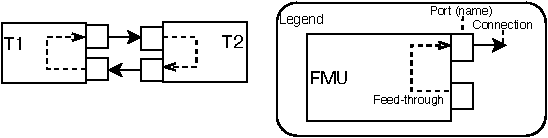
\includegraphics[width=1\textwidth]{images/fmu_cycle.pdf}
    \end{minipage}\hfill
    \begin{minipage}{0.35\textwidth}
        \centering
    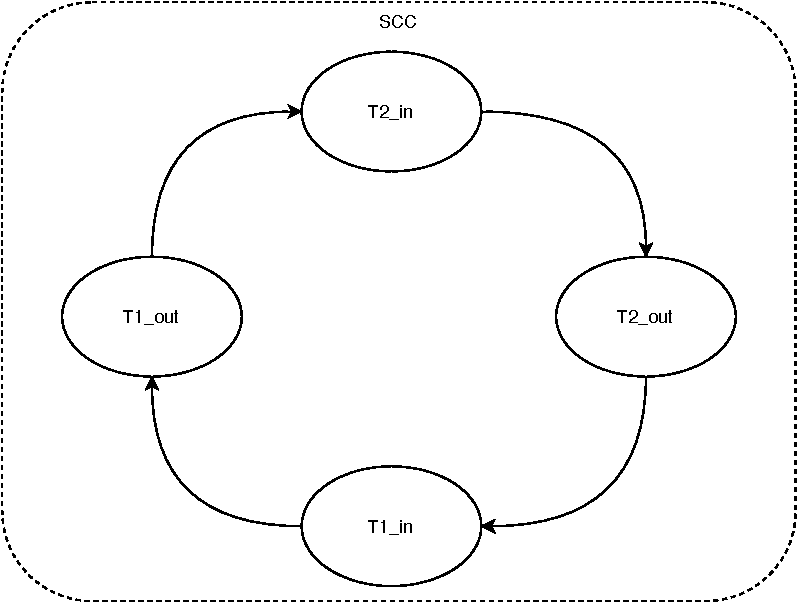
\includegraphics[width=1\textwidth]{images/SCC.pdf}
    \end{minipage}
    \caption{An FMU co-simulation scenario and its Initialization Graph}
    \label{fig:fmu_cycle}
\end{figure}


The following definitions formalizes the concept of an algebraic loop in a co-simulation scenario, and define the problem these algebraic loops are introducing.
The definition of strongly connected components is adapted from the semantics of Causal Block Diagrams (see \cite{Gomes2020} for an overview).

\begin{definition}[Algebraic loops] 
An algebraic loop is defined as a non-trivial strongly connected component of the graph in \cref{def:initialization_graph}.
Formally, a strong connected component satisfies $\set{a,b \in SCC: \mathit{Path}(a,b)}$, where $\mathit{Path}(a,b)$ is true when there's a path (including an empty path) between nodes $a$ and $b$ ($\mathit{Path}(a,a)$ is always true).
An $SCC$ is non trivial when it has more than one node.
%$\LoopVariables = \{v | v \in V : Path(v,v)\}$ \\
%An algebraic loop is defined as the set $\{p_1, p_2 | p_1, p_2 \in \LoopVariables: Path(p_1, p_2) \land Path(p_2, p_1)\}$/
%Path is defined as the transitive closure of the edges of the graph denoted by \cref{def:initialization_graph}.
\end{definition}

Since the edges of the graph represent dependencies between variables, the value of every variable in a non trivial strong component depends on itself.
Let $X$ denote a vector of one or more variables whose value depends on itself. Then the non trivial strong component forms an equation with the form $F(X, U) = X$, where $F$ denotes the relations between the variables in the loop, and $U$ denotes the variables whose values are calculated elsewhere.
This means that algebraic loops need to be handled using fixed point iterations\cite{Gomes2018}. 
% It is a technique to repeatedly perform the steps of a sub-list of the co-simulation step. The number of repetitions the operations should be performed depends on the characteristics of the scenario. The operations should be performed until the system converge. 
An example of applying a fixed point iteration can be seen in \cref{def:fixedpoint} where a system containing an algebraic loop has to be initialized using fixed point iteration.
\claudio{Perhaps later you can ditch \cref{fig:fixedpont} and refer to the case study section, to shorten the text.}
\claudio{You should avoid forcing Latex to position pictures in a particular place. It's bad practice because it causes too much blank space. Also it's a lot of work for you to care about the specific placement of figures.}

\begin{figure}
    \centering
    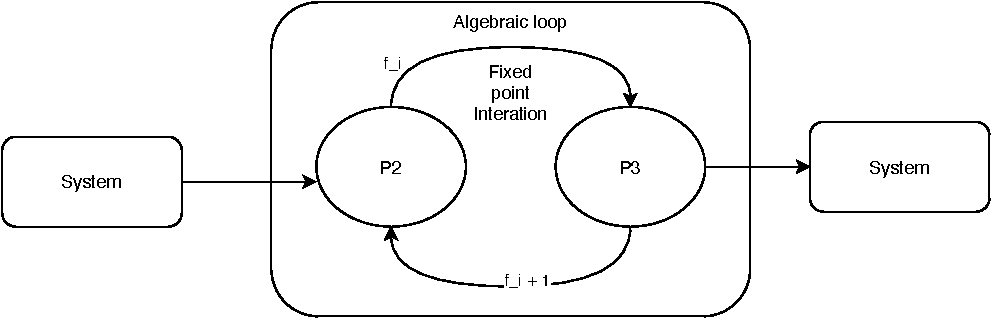
\includegraphics[width=0.8\textwidth]{images/fixedpoint.pdf}
    \caption{Fixed point iteration in a co-simulation scenario}
    \label{fig:fixedpont}
\end{figure}

% The initialization of the system requires the application of fixed point iteration, as defined \cref{def:fixedpoint}.
\begin{definition}[Fixed point iteration of an Initialization procedure]\label{def:fixedpoint}
A fixed point iteration of given loop $l$ consist of the order sequence of functions calls:
$\forall v \in l: \exists op \in \fixedpoint{l} : op = \fget{}(\dontcare, v) \lor op = \fset{}(\dontcare, v, \dontcare)$.
Performing a iteration on a co-simulation state leads to a new state to $\fixedpoint{l}(\state{n}) = \state{n + 1}$
The fixed point iteration is performed in order to find a convergent initialization state as defined in \cref{def:convergence}.
\end{definition}

\claudio{The above defintions is strange. If there's an algebraic loop, you cannot have an initialization procedure. At least not the way it is currently defined. Also I feel that you don't really need to define the fixed point iteration. We just need to reformulate the initialization procedure so that it matches what your plugin should output.}

A fixed point iteration technique is not guaranteed to convergence if the system is unstable. This means that an upper bound of the number of repetitions needs to be established to ensure termination. In case of a non-converging algebraic loop the simulation should be stopped since the result of the co-simulation scenario would not be trustworthy. The criteria of a valid co-simulation scenario is specified in \cref{def:convergence}.

\begin{definition}[Convergence of Fixed point iteration]\label{def:convergence}
A fixed point iteration converges if a finite number of iterations will make the difference of the output value of the same operation between two following iterations within a certain threshold $\epsilon$.\\
Formally, 
$\exists n \in \setnat: |F(X^{n+1}, U) - F(X^{n}, U)| \leq \epsilon$.
\end{definition}

\subsection{INTO-CPS Maestro 2}\todo{We can have some more in this section - Ask Casper if he can do it?}
INTO-CPS Maestro 2\footnote{currently in alpha \url{https://github.com/INTO-CPS-Association/maestro/tree/2.0.0-alpha}}\cite{Thule2019b} is an FMI-based co-simulation framework set to supersede Maestro\cite{Maestro}. The philosophy of the framework is to apply plugins to generate co-simulation specifications expressed in the domain specific language called Maestro Base Language (MaBL). Such specifications are then interpreted and executed, resolving in the execution of a co-simulation.

\section{Calculation of an Initialization Order}\label{sc:initilization}
The FMI specification defines certain information about the initialization order described through different states of a co-simulation. The initialization phase covers the two states (in chronological order) defined in the specification:
\begin{itemize}
    \item \textit{Instantiated}
    \item \textit{Initialization Mode}
\end{itemize}
In each of the two states, different groups of FMU variables and parameters are potentially assigned a value. The groups are defined by FMI based on rules of the characteristics of the variables. These rules have been extracted as predicates and used in the implementation. 
Some groups consist of variables and parameters whose value does not depend on other variables. These can be set before entering the \textit{Initialization Mode}. Since these variables have no connections to other FMU variables - meaning they are not represented in the graph of \cref{def:initialization_graph}, the order is insignificant. 
The setting and getting operations are of each FMU are grouped to perform the fewest possible operations in the initialization. 

In the \textit{Initialization Mode} state, all variables of all FMUs should be defined.
The parameters of each FMU are set first, and the order in which they are set is again insignificant as they are independent.
Afterwards the interconnected variables should be defined, but as stated by the \cref{def:feedthrough,def:getout,def:setin} the operations \textit{get} and \textit{set} \textbf{require} a specific initialization order, and algebraic loops place even more requirements on the initialization strategy. Since each non-trivial strongly connected component needs to be isolated from the other variables of the system to obtain their initial values using fixed point iteration. 

%\%claudio{I feel like the previous two sentences are a bit contradictory, and are probably constructed like so because you did not deal with algebraic loops upfront. When algebraic loops are not there, there must be an order. But when algebraic loops are there, it's not that there's more constraints... it's just that one has to isolate the strong components from the rest. The result is then an order between strongly connected components, but no order within each component}

\subsection{Method to calculate the initialization order}
This section describes the approach taken to calculate the initialization order of the interconnected FMU variables. The approach is based on the strategy proposed in Gomes et al. \cite{Gomes2019b, BromanCompositionCo-Simulation}, but the approach in this work is extended with the ability to handle the initialization of algebraic loops. 

%\claudio{I like the way in which you've structured this subsection... but perhaps you don't need to make this structure explciit in the latex.. just leave the subsubsection comments commented out, but still follow the structure.}
%\subsubsection{Structure of the graph}
The initialization algorithm starts by building a directed graph of the dependency between the interconnected variables of the FMUs. The graph is constructed based on the interconnected variables and internal connections (feed-through), as in \cref{def:initialization_graph}. 
%Each interconnected variable in the system represents a node, and the edges are based on these connections. The edges of this graph represent precedence constraints based on the algebraic dependencies of the interconnected variables. Please see \cref{def:initialization_graph} for a formal definition of the graph.

%As described earlier, not all co-simulation scenarios are suitable, and these invalid scenarios need to be identified in this phase to avoid wasting valuable development. This is accomplished by monitoring convergence of all algebraic loops. A valid co-simulation scenario must convergence by \cref{def:convergence}.
%\claudio{Wait a second... you can only monitor convergence once you have an initialization order, and you start solving the loops. Why is paragraph here if the calculation of an initialization order is still to be explained? Maybe move this explanation to after that part.}

%\subsubsection{Calculation of an initialization order}
The topological ordering of the strongly connected components of the graph defined in \cref{def:initialization_graph} is the initialization order of the interconnected FMU variables. 
The non-trivial strongly connected components are algebraic loops of the system. The trivial ones are standard interconnected FMU variables, whose port operation should be performed only once during the initialization procedure.
The calculation of an initialization order is performed in linear time based on the number of both external and internal connections using Tarjan's algorithm \cite{tarjan_1972}. 
%This algorithm is selected due to its properties. It solves two of the central issues of the initialization-phase of the co-simulation.
%\begin{itemize}
%    \item Identifies algebraic loops between interconnected variables (strongly connected components)
%    \item Performs a topological sorting of the Strongly Connected Components
%\end{itemize}
The algorithm is well-established, and there exist formal proofs of its correctness and properties\cite{stefanMerz}. 
% The algorithm is among the most efficient graph algorithms for accomplishing the defined goals.
% Tarjan's algorithm is performing a topological sorting of the strongly connected components of a graph. Moreover, it can handle both graphs with and without algebraic loops.

%\subsubsection{Handling of algebraic loops}
As described in earlier sections, it is essential to handle the algebraic loops by a particular initialization strategy since they otherwise would invalidate the result of the co-simulation. The strategy for managing algebraic loops is to identify and initialize them using a fixed point iteration until convergence. Since convergence is not guaranteed, this property is monitored using \cref{def:convergence}. If convergence is not established within a finite number of iteration, the co-simulation is rejected to avoid running an invalid simulation.

\subsection{Optimization of a Initialization Procedure}
An initialization procedure can be optimized since the FMI specification allows multiple \textit{set} or \textit{get} operations of the same FMU to be performed in bulk by grouping them together to a single operation over multiple variables with similar characteristic. This criteria of optimization is formalized in \cref{def:optimization}
\begin{definition}[Optimization of a Initialization procedure]\label{def:optimization}
  Given an initialization procedure $\sequence{\initcall_i}_{i \in \setnat}$ with a finite ordered sequence of FMU function calls $\functioncall_i \in \allfunctioncalls = \bigcup_{c \in \fmus} \set{\fset{c},\fget{c}},$ and $i$ denoting the order of the function call. It can be optimized if $\exists \functioncall_i, \functioncall_{i +1} \in \allfunctioncalls : \exists c \in \fmus :(\functioncall_i \in {\fset{c}} \land \functioncall_{i+1} \in {\fset{c}}) \lor (\functioncall_i \in {\fget{c}} \land \functioncall_{i+1} \in {\fget{c}})$
\end{definition}
%Since an Initialization procedure is defined in the same way as other co-simulation steps (see \cref{def:initialization}), the optimization criteria described in \cref{def:optimization} is valid for an arbitrary co-simulation step. \\
The correctness of the optimization in \cref{def:optimization} is established by the proof of using the Initialization Graph's topological ordering as the initialization order by Gomes et al. \cite{Gomes2019}. This proof is valid for this approach since the optimization does not change the structure of the Initialization Graph. \\
A limitation of this optimization strategy is that it is not guaranteed to find all potentially valid optimizations of a co-simulation scenario. Considering it works only on a specific co-simulation step (a topological order of a graph), which is not necessarily unique for a given co-simulation scenario. A more advanced optimization strategy needs to be developed to perform all viable optimizations of a co-simulation step. Another solution is to apply this optimization strategy on the set of all valid co-simulation steps - yielding a potential very inefficient initialization algorithm.

\subsection{The entire Initialization Strategy}
The pseudo-code in \cref{alg:initialization} formulates the entire initialization strategy of the interconnected variables of a co-simulation scenario.
\begin{figure}[H]
  \centering
    \begin{algorithm}[H]
    \caption{Initialization strategy for Interconnected variables}
    \label{alg:initialization}
      \begin{algorithmic}[1]
        \State $InitializationGraph \gets createGraph(connections)$
        \State $SCCS \gets Tarjan(InitializationGraph)$
        \State $OptimizeInitializationOrder(SCCS)$
        \ForEach {$SCC \in SCCS$}
            \If {$isAlgebraicLoop(SCC)$}
                \State $applyFixedPointIteration(SCC)$;
            \Else
                \State $initializeVariable(SCC)$;
            \EndIf
        \EndFor
        \end{algorithmic}
    \end{algorithm}
\end{figure}

\section{Case study}

%This paper's main contribution is to calculate an initialization order of a co-simulation scenario potentially containing algebraic loops. The approach make the circular dependencies between the interconnected converge in the initialization, so the initial values of the interconnected variables in the system being simulated is stable at the time the co-simulation is started.

In this section, we give a simple example of a co-simulation whose correct initialization demands the solution to an algebraic loop.

In the example case study, the acceleration can be set to 0, at time 0.
We show that \verb|tire_x| depends on itself as a consequence:
\begin{verbatim}
0 = a = (1/tire_mass) * F_total
0 = F_total = F_rubber + F_suspension - f_gravity
f_gravity - F_suspension = F_rubber
F_rubber = - rubber_stiffness*tire_x - rubber_damping * tire_v
tire_v = 0
F_rubber = - rubber_stiffness*tire_x

F_suspension = suspension_stiffness*(car_x - tire_x) + suspension_damping*(car_v - tire_v);

tire_x = F(F_rubber) = G(F_suspension)= H(tire_x)
\end{verbatim}


\section{Realization of a Maestro 2 Plugin}\label{sc:implementation}
This approach has been realized as a Maestro 2 plugin that generates the \textit{Initialization}-phase of a co-simulation specification expressed in MaBL. It calculates the specification based on a list of FMU-components of a co-simulation scenario, and a specific plugin-configuration to let the user supply initial values of FMU variables with $causality=parameter$. A correction initialization specification can be calculated by the plugin if the co-simulation scenario is adhering to the behavior dictated by definition given in \ref{def:convergence}.

The plugin optimizes the initialization order by grouping operations that can be executed in \textit{parallel} to take advantage of FMI's ability to \textit{set} or \textit{get} multiple variables in bulk from the same FMU. The criteria for this optimization is defined in definition \ref{def:optimization}. 
The developed plugin has been tested on numerous co-simulation examples from the INTO-CPS universe\cite{Maestro} and compared with the existing \textit{Initializer} of Maestro. The plugin has been tested in the whole Maestro 2 pipeline to practically verify that it can be used in a co-simulation where the generated initialization procedure is integrated as a part of a complete co-simulation to verify the initialization procedure's integration with a master algorithm.

\subsection{Realization of the Topological Sorting}
The topological sorting algorithm (Tarjan's Algorithm) is implemented in Scala. The motivation for choosing Scala is its relation to JVM and the connection to Slang and the Logika framework\cite{inbook}. The connection to Slang and Logika will be investigated in the future. The Logika framework will be used to formally verify the implemented plugin and be used to explore how the contract-based nature of Slang can be used to obtain more reliable results of co-simulations. The topological sorting returns a topological order of strongly connected components. This order is the order of initialization, where the elements containing more than a single element denotes an algebraic loop that requires a particular initialization strategy. 

\subsection{Verification of the Initialization Order}
The realized plugin is verified in several ways using traditional proof methods and practical verification against an established co-simulation Verifier. The approach behind the plugin has been verified by Gomes et al. that in \cite{gomes_lucio_vangheluwe_2019} proved the correctness of using the topological order of a dependency graph of the interconnected variables to generate for the order of the operations that need to be performed in a co-simulation step (both the initialization procedure and an arbitrary step). Gomes et al. used a graph based on FMU-operations (\textit{Set, Get, doStep}) instead of interconnected variables, which is the approach described in this paper. The simplification of using the interconnected variables is valid since this approach only cares about initialization and, therefore, does not need to care about the time of each FMU. This does that we can omit all the \textit{doStep} nodes, it means that each interconnected variable can only perform one of the two operations \textit{get} or \textit{set} as described by the definitions \ref{def:getout} and \ref{def:setin}.
This approach does, therefore, end up with a subgraph of the graph by Gomes et al. The proof from \cite{gomes_lucio_vangheluwe_2019} can trivially be modified to the graph/approach presented in this paper.

\subsubsection{Practical verification against a Verifier} 
Gomes et al.'s main contribution is an implementation of the criteria for a valid FMI based co-simulation formulated in Prolog freely available to be used in other projects\footnote{\url{http://msdl.cs.mcgill.ca/people/claudio/projs/PrologCosimGeneration.zip}}. The Prolog implementation was used in their research to verify their approach for generating co-simulation algorithms formally. The Prolog realization encapsulates all the rules of a valid co-simulation step (both master-algorithm and an initialization algorithm). 
This work includes an integration from the developed plugin to the Prolog Verifier. The integration has been realized to systematically verify the correctness of the calculated initialization order against an established and recognized co-simulation Algorithm Verifier. The integration queries the Prolog database with a co-simulation environment and a calculated initialization order to verify the order's correctness. The integration performs all the necessary transformations of the dependency graph (see definition \ref{def:initialization_graph}) used in the Maestro plugin to a graph of FMU operations used in the Prolog database. The transformation is based on the definitions \ref{def:getout} and \ref{def:setin}. The Prolog integration is not applied if the graph contains algebraic loops since the Prolog database does not support these scenarios.

The Prolog code is capable of generating a valid initialization order, but this functionality is not used for several reasons. The main reasons are based on performance considerations and the desire to handle the initialization of co-simulation scenarios containing strongly connected components.

\section{Related Work}
Prior work \cite{Gomes2019, BromanCompositionCo-Simulation} is looking into the generation of co-simulation algorithms (both master and initialization algorithms) for FMI-based scenarios. Their generation technique is like ours based on a dependency graph of the operations of a co-simulation step. Both Gomes and Broman present an approach for using the topological order of a dependency graph to establish a correct order of operations in a co-simulation step of a given co-simulation scenario.
The work by Gomes et al. \cite{Gomes2019} does also define the criteria for a correct co-simulation step. Their work has many similarities with ours. However, their work is mostly concerned with the theoretical aspect of co-simulation algorithm generation and verification, while our work has a more practical nature. Gomes et al. do also not consider the handling of algebraic loops, which is a key feature of our approach. Furthermore, the approach taken in our work is only concerned with the initialization procedure of a co-simulation.

Broman et al. \cite{BromanCompositionCo-Simulation} also suggest to use the topological sorting of a dependency graph of the interconnected variables to detect algebraic loops and discover the partial order of port-operations. Nevertheless, they explicitly specify the requirement for cycle freedom in the dependency graph as a precondition for the generation of a valid co-simulation. It means they refuse all co-simulation scenarios containing algebraic loops. It is a significant difference to our approach that applies a fixed point iteration strategy to handle these scenarios. Also, the approach in this paper is more specialized because it only considers the initialization of a co-simulation, which means it deals with non-interconnected variables.

Amalio et al. \cite{Amalio2016CheckingCo-simulation} investigate how to avoid algebraic loops in FMU based co-simulation scenarios by statically checking the architectural design of a CPS. The publication's purpose is like ours to avoid invalid co-simulation scenarios. Nevertheless, they achieve this by excluding co-simulation scenarios containing algebraic loops. Their method is realized in a co-simulation tool, INTO-SysML\cite{Miyazawa2016INtegratedModelling}. Formal methods form the basis of their work (Theorem Proving and Model-checking). It will be an inspiration for the future work of formally verifying the plugin and other parts of Maestro 2. 

The work by \cite{EvoraGomez2019a} in of a similar nature to ours. They use Tarjan’s SCC algorithm to generate a sorted DAG of strongly connected components to solve the initialization problem.
Even though their work is very similar to ours, we extend their approach with a verification against the simulation semantics resulting in a formal more sounds approach. However further work will look into further improvements and formal verification of the current approach.

\section{Concluding remarks}\label{sc:summary}
This work uses a topological ordering of a dependency graph of the interconnected FMUs variable and internal FMU variable connections along with predicates from the FMI specification to calculate a correct initialization order for a co-simulation scenario. The plugin optimizes the calculated initialization order by grouping variables with similar characteristics to perform the fewest possible operations in the initialization procedure.
This approach supports the initialization of a co-simulation scenario containing algebraic loops by utilization of fixed point iteration. The approach discards all co-simulation scenarios, not adhering to the law of convergence \ref{def:convergence}.
It is possible to combine the approach with an arbitrary master algorithm to run a co-simulation. \\
The approach is realized as a plugin for the open-source INTO-CPS Maestro 2 tool and verified against the existing \textit{Initializer} and the calculated initialization order was verified against an established co-simulation Algorithm Generator and Verifier implemented in Prolog\cite{gomes_lucio_vangheluwe_2019}\\
Future work includes formal verification of the plugin using the Logika framework\cite{inbook}.
We will also look into the generation of a verification strategy for the whole Maestro 2 framework to examine how different forms of verification jointly can extend the trust of the correctness of the result of a co-simulation. 

\paragraph*{\textbf{Acknowlegements.}}We would like to thank Stefan Hallerstede, Christian Møldrup Legaard, and Peter Gorm Larsen for providing valuable input to this paper and the developed plugin.
%
% ---- Bibliography ---

\bibliographystyle{splncs04}
\bibliography{gen_bib,gen_bib_claudio}


\end{document}
